% Generated by book/tools/notebook_to_tex.py. Do not edit by hand.

\chapter[GPT-2 계속 사전학습 (Continual Pretraining)]{GPT-2 계속 사전학습 (Continual Pretraining)}

\label{ch:25}

\markboth{GPT-2 계속 사전학습 (Continual Pretraining)}{GPT-2 계속 사전학습 (Continual Pretraining)}

\chaptermeta{25_gpt2_continual_pretrain/25_gpt2_continual_pretrain.ipynb}{https://colab.research.google.com/github/yoon-gu/neuqes-101/blob/master/25_gpt2_continual_pretrain/25_gpt2_continual_pretrain.ipynb}{OpenAI gpt2를 같은 TinyStories 데이터로 continual pretraining하며 scratch pretraining과 비교}



\index{1GPT 2@GPT-2}

\index{1continual pretraining@continual pretraining}

\index{1continual learning@continual learning}

\index{1AutoModelForCausalLM@AutoModelForCausalLM}

\index{1AutoTokenizer@AutoTokenizer}

\index{1gpt2@gpt2}

\index{1WebText@WebText}

\index{1catastrophic forgetting@catastrophic forgetting}

\index{1learning rate@learning rate}

\index{1gradient accumulation@gradient accumulation}

\index{1CausalLM@CausalLM}

\index{1DataCollatorForLanguageModeling@DataCollatorForLanguageModeling}

\index{1labels 100@labels=-100}

\index{1TinyStories@TinyStories}

\index{1generation comparison@generation comparison}

\index{0계속 사전학습@계속 사전학습}

\index{0연속 학습@연속 학습}

\index{0파국적 망각@파국적 망각}

\index{0학습률@학습률}

\index{0그래디언트 누적@그래디언트 누적}

\index{0생성 비교@생성 비교}

\index{0사전학습 본체@사전학습 본체}

\index{1AutoModelForCausalLM from pretrained@AutoModelForCausalLM.from\_pretrained}

\index{1AutoTokenizer from pretrained@AutoTokenizer.from\_pretrained}

\index{1tokenizer pad token@tokenizer.pad\_token}

\index{1eos token@eos\_token}

\index{1WebText pretraining@WebText pretraining}

\index{1learning rate 2e 5@learning\_rate=2e-5}

\index{1gradient accumulation steps@gradient\_accumulation\_steps}

\index{1effective batch@effective batch}

\index{1domain adaptation@domain adaptation}

\index{1continual pretraining loss@continual pretraining loss}

\index{1Ch 24 vs Ch 25@Ch 24 vs Ch 25}

\index{1scale effect@scale effect}

\index{1pretraining effect@pretraining effect}

\index{1SFT boundary@SFT boundary}

\index{1prompt masking@prompt masking}

\index{0도메인 적응@도메인 적응}

\index{0효과적 배치@효과적 배치}

\index{0본체 출발점@본체 출발점}

\index{0스케일 효과@스케일 효과}

\index{0사전학습 효과@사전학습 효과}

\index{0SFT 경계@SFT 경계}

\index{0프롬프트 마스킹@프롬프트 마스킹}



\section{누적 추적표}

\begin{booktable}{25장 누적 추적표 표}{tab:ch25-01}
\begin{adjustbox}{max width=\textwidth}
\begin{tabular}{@{}llllll@{}}
\toprule
Ch & 모델 & 토크나이저 & 데이터 & Output Head & Loss \\
\midrule

22 & 작은 BERT (한국어, scratch) & \inlinecode{klue/bert-base} (가져옴) & 한국어 위키 paragraphs & MLM head & \inlinecode{CrossEntropyLoss} (masked 15\%) \\
23 & \ref{ch:22}장 + 분류 헤드 & (\ref{ch:22}장과 동일) & NSMC 이진 & \inlinecode{Linear(H,\ 2)} & \inlinecode{CrossEntropyLoss} \\
24 & 작은 GPT2 (직접, scratch, 약 3M) & BPE (직접 학습, vocab 2,048) & TinyStories 30K & \inlinecode{Linear(H,\ V)} (LM head, weight tied) & \inlinecode{CrossEntropyLoss} (next-token) \\
\textbf{25 \(\leftarrow\) 여기} & \textbf{\inlinecode{gpt2} (124M, OpenAI WebText 사전학습)} & \textbf{BPE (gpt2 그대로, vocab 50,257)} & \textbf{TinyStories 30K (\ref{ch:24}장과 동일)} & \textbf{\inlinecode{Linear(H,\ V)} (LM head 그대로)} & \textbf{\inlinecode{CrossEntropyLoss} (next-token) --- \emph{continual pretraining}} \\
26 (다음) & 작은 GPT (한국어, scratch) & BPE (한국어 직접 학습) & 한국어 TinyStories-Korean & \inlinecode{Linear(H,\ V)} (LM head, weight tied) & \inlinecode{CrossEntropyLoss} (next-token) \\
\bottomrule
\end{tabular}
\end{adjustbox}
\end{booktable}

전체 장 표는 \href{https://github.com/yoon-gu/neuqes-101\#챕터별-변화추적표}{루트 README} 를 참고하세요.

\begin{center}\rule{0.5\linewidth}{0.5pt}\end{center}

\subsection{\texorpdfstring{\ref{ch:24}장 \(\leftrightarrow\) \ref{ch:25}장 격리 실험의 통제 변수}{\ref{ch:24}장 \textbackslash leftrightarrow \ref{ch:25}장 격리 실험의 통제 변수}}

\begin{booktable}{25장 24장 \ensuremath{\leftrightarrow} 25장 격리 실험의 통제 변수 표}{tab:ch25-02}
\begin{adjustbox}{max width=\textwidth}
\begin{tabular}{@{}llll@{}}
\toprule
항목 & \ref{ch:24}장 & \textbf{\ref{ch:25}장 (본 장)} & 같음 / 다름 \\
\midrule

데이터 & TinyStories 30K & TinyStories 30K & \textbf{같음} (통제 변수) \\
Trainer 클래스 & \inlinecode{transformers.Trainer} & \inlinecode{transformers.Trainer} & \textbf{같음} \\
Data collator & \inlinecode{DataCollatorForLanguageModeling(mlm=False)} & \inlinecode{DataCollatorForLanguageModeling(mlm=False)} & \textbf{같음} \\
Loss & CE next-token (\inlinecode{labels\ =\ input\_ids.clone()}) & CE next-token (\inlinecode{labels\ =\ input\_ids.clone()}) & \textbf{같음} \\
본체 출발점 & \inlinecode{GPT2LMHeadModel(config)} random init (3M) & \inlinecode{AutoModelForCausalLM.from\_pretrained("gpt2")} (124M) & \textbf{다름} \\
토크나이저 & BPE 직접 학습 (vocab 2,048) & \inlinecode{AutoTokenizer.from\_pretrained("gpt2")} (vocab 50,257) & \textbf{다름} (본체와 운명공동체) \\
학습률 & 3e-4 (scratch 표준) & \textbf{2e-5} (continual pretraining 표준) & \textbf{다름} \\
학습 step & 약 1,500 & \textbf{약 3,200} (51,863 chunks / eff. batch 16, 1 epoch) & \textbf{다름} (lr 만 작아짐) \\
\bottomrule
\end{tabular}
\end{adjustbox}
\end{booktable}

\begin{quote}
\textbf{세 줄 차이가 곧 \emph{학습 단계 2 (continual pretraining)} 의 정의} --- 같은 task, 같은 collator, 같은 loss, 같은 trainer. \emph{모델 로드 한 줄 + 토크나이저 한 줄 + lr 한 숫자} 만 바꾸면 됩니다.
\end{quote}



\section{변경점: \ref{ch:24}장 대비}

\begin{booktable}{25장 변경점 요약}{tab:ch25-03}
\begin{adjustbox}{max width=\textwidth}
\begin{tabular}{@{}lll@{}}
\toprule
축 & \ref{ch:24}장 (영어 GPT scratch) & \ref{ch:25}장 (본 장, gpt2 continual pretraining) \\
\midrule

\textbf{본체} & 작은 GPT2 (약 3M params, random init) & \textbf{\inlinecode{gpt2}} (124M, OpenAI WebText 약 40GB 사전학습) \(\leftarrow\) \emph{출발점 변화} \\
\textbf{토크나이저} & BPE 직접 학습 (vocab 2,048) & \textbf{\inlinecode{AutoTokenizer.from\_pretrained("gpt2")}} (vocab 50,257) \(\leftarrow\) \emph{본체에 맞춰 함께 변함} \\
데이터 & TinyStories 30K & \textbf{TinyStories 30K (동일)} \(\leftarrow\) 통제 변수 \\
Trainer & \inlinecode{transformers.Trainer} & \textbf{\inlinecode{transformers.Trainer} (동일)} \\
Data collator & \inlinecode{DataCollatorForLanguageModeling(mlm=False)} & \textbf{(동일)} \\
Loss & CE next-token (\inlinecode{labels\ =\ input\_ids.clone()}) & \textbf{(동일)} \\
\textbf{학습률} & 3e-4 & \textbf{2e-5} \(\leftarrow\) \emph{유일한 hyperparam 큰 차이} \\
학습 step & 약 1,500 (T4 약 1분) & \textbf{약 3,200 (T4 약 19분)} --- 124M 본체라 step 당 비용이 큼 \\
Generation 품질 & grammatical 한 동화 풍 & \textbf{자연스러운 동화 + 일반 도메인 폭} \(\leftarrow\) 메시지 \\
\bottomrule
\end{tabular}
\end{adjustbox}
\end{booktable}

\begin{quote}
\textbf{핵심}: \emph{\ref{ch:24}장 \(\leftrightarrow\) \ref{ch:25}장은 데이터·trainer·collator·loss 모두 같고 본체 출발점·토크나이저·lr 만 다름}. \textbf{trainer 코드 차이가 극단적으로 적음} --- 그게 GPT 시대 학습 단계 2 (continual pretraining) 의 본질. \emph{task adaptation 의미의 fine-tune 이 아닙니다} --- head 바뀌지 않고, task (next-token 예측) 바뀌지 않습니다. 데이터만 바뀝니다.
\end{quote}



\section{GPT 시대 학습 4단계 --- 본 장의 위치 (단계 2)}

\ref{ch:24}장에서 도입한 GPT 시대 학습 4단계 표의 \emph{단계 2 (continual pretraining)} 가 본 장입니다.

\begin{booktable}{25장 GPT 시대 학습 4단계 - 본 장의 위치 (단계 2) 표}{tab:ch25-04}
\begin{adjustbox}{max width=\textwidth}
\begin{tabular}{@{}llllll@{}}
\toprule
단계 & 정확 용어 & 의미 & \inlinecode{labels\ =\ -100} 자리 & 본 커리큘럼 & 본 장? \\
\midrule

1 & \textbf{Pretraining} (사전학습) & 일반 코퍼스 위에 random init 본체부터 학습 & pad 만 & \ref{ch:24}장, \ref{ch:26}장 & \\
2 & \textbf{Continual pretraining} (계속 사전학습 / continual learning) & \emph{사전학습된 본체} 를 \emph{새 데이터} 로 \emph{같은 CausalLM task} 더 학습. \textbf{head 그대로, task 그대로, 데이터만 새로} & pad 만 (단계 1 과 동일) & \textbf{\ref{ch:25}장 \(\leftarrow\) 여기} & OK \\
3 & \textbf{SFT} (Supervised Fine-Tuning / Instruction tuning) & instruction-response 쌍으로 \emph{행동 정렬}. \texttt{labels{[}:prompt\_len{]}\ =\ -100} 으로 답변 부분만 학습 & \textbf{prompt 부분} & \ref{ch:28}장 & \\
4 & \textbf{Alignment} (DPO / RLHF / GRPO) & preference 또는 verifier reward 로 \emph{선호 정렬} & (RL 내부) & \ref{ch:30}--\ref{ch:31}장 & \\
\bottomrule
\end{tabular}
\end{adjustbox}
\end{booktable}

\subsection{\texorpdfstring{\ref{ch:25}장은 \emph{SFT 가 아닙니다}}{\ref{ch:25}장은 SFT 가 아닙니다}}

본 장을 \emph{fine-tune} 으로 부르면 \emph{단계 2 / 3 / 4} 가 모두 섞여 혼동이 생깁니다. \ref{ch:25}장의 정확한 위치는:

\begin{itemize}
\tightlist
\item
  \textbf{\inlinecode{task\ adaptation} 의미의 fine-tune 이 아님} --- output head 안 바뀜 (LM head 그대로), task 안 바뀜 (next-token 예측 그대로), loss 안 바뀜 (CE)
\item
  \textbf{\inlinecode{instruction\ tuning} 의미의 SFT 가 아님} --- \inlinecode{labels\ =\ -100} 자리가 \emph{pad 만} (\ref{ch:24}장과 동일). prompt-response 쌍 데이터 형식이 아니라 \emph{연속된 일반 텍스트}
\item
  \textbf{\inlinecode{continual\ pretraining} 그 자체} --- \emph{사전학습된 본체 + 새 도메인 데이터 + 같은 CausalLM task} 의 조합. \emph{데이터만 바뀐 단계 1 의 연장}
\end{itemize}

\begin{quote}
SFT (단계 3) 는 \ref{ch:28}장에서 본격. \emph{왜 모델이 instruction 을 따라가게 되는가} 는 \texttt{labels{[}:prompt\_len{]}\ =\ -100} 한 줄로 정확히 설명됩니다. 본 장의 collator 출력 (거의 모든 자리 = 학습 신호) 이 그 한 줄과 정확히 대비되는 \emph{학습 단계 2 의 기준선}.
\end{quote}



\section{\texorpdfstring{Loss --- 변화 없음, 다만 \emph{시작점} 이 다름}{Loss --- 변화 없음, 다만 시작점 이 다름}}

\ref{ch:24}장과 \emph{완전히 동일} 한 \inlinecode{CrossEntropyLoss} (next-token, \inlinecode{mlm=False}). \inlinecode{labels\ =\ input\_ids.clone()}, pad 만 \inlinecode{-100}. 단 \emph{vocab 차원이 2,048 \(\to\) 50,257 로 커진} 영향과, \emph{모델 본체가 random init 이 아닌 이미 학습된 상태} 라는 두 차이가 \emph{loss 곡선의 시작 지점} 을 결정합니다.

\subsection{Random baseline 의 변화}

\begin{booktable}{25장 Random baseline 의 변화 표}{tab:ch25-05}
\begin{adjustbox}{max width=\textwidth}
\begin{tabular}{@{}llll@{}}
\toprule
토크나이저 & vocab 차원 & \inlinecode{ln(vocab)} (uniform CE) & 장 \\
\midrule

직접 학습 BPE & 2,048 & 7.62 & \ref{ch:24}장 \\
\textbf{gpt2 BPE} & \textbf{50,257} & \textbf{10.82} & \textbf{\ref{ch:25}장} \\
\inlinecode{klue/bert-base} WordPiece & 32,000 & 10.37 & \ref{ch:22}--\ref{ch:23}장 (참고) \\
\bottomrule
\end{tabular}
\end{adjustbox}
\end{booktable}

\emph{만약} gpt2 본체가 random init 이었다면 첫 step loss 가 약 10.82 부근에서 시작할 것입니다. 하지만 \textbf{gpt2 본체는 이미 WebText 약 40GB 로 사전학습되어 있어} \emph{TinyStories 평가에서도 시작 loss 가 random baseline 보다 훨씬 낮습니다} --- 그게 학습 단계 2 의 핵심 차이.

\subsection{\texorpdfstring{숫자로 감 잡기 --- \emph{시작점 \(\leftrightarrow\) 도달점}}{숫자로 감 잡기 --- 시작점 \textbackslash leftrightarrow 도달점}}

\begin{booktable}{25장 숫자로 감 잡기 - 시작점 \ensuremath{\leftrightarrow} 도달점 표}{tab:ch25-06}
\begin{adjustbox}{max width=\textwidth}
\begin{tabular}{@{}lll@{}}
\toprule
상태 & 정답 토큰 확률 & \(-\log p\) \\
\midrule

균등 추측 (gpt2 vocab 50,257) & \(1/50257\) & \textbf{10.82} \(\leftarrow\) random baseline (도달 불필요) \\
gpt2 사전학습 그대로, TinyStories 평가 & \(0.05\) - \(0.10\) 범위 & \textbf{2.5 - 3.0} \(\leftarrow\) \emph{우리 시작점} (이미 좋음) \\
Continual pretraining 후 (수백 step) & \(0.10\) - \(0.20\) 범위 & \textbf{1.6 - 2.3} \(\leftarrow\) \emph{우리 도달점} \\
Reference: 학습 길게 했을 때 & \(0.25\)+ & 약 1.4 \\
\bottomrule
\end{tabular}
\end{adjustbox}
\end{booktable}

\begin{quote}
\ref{ch:24}장의 시작 loss \inlinecode{약\ 7.6} (random baseline) 와 \ref{ch:25}장의 시작 loss \inlinecode{약\ 2.5-3.0} (사전학습된 본체의 평가 loss) 의 차이가 \emph{대규모 사전학습이 본체에 미리 새겨둔 next-token 분포} 의 정량적 가치. \emph{\ref{ch:25}장은 random 에서 시작하지 않습니다}.
\end{quote}

\subsection{Perplexity 환산}

\(\text{PPL} = e^{L}\):

\begin{booktable}{25장 Perplexity 환산 표}{tab:ch25-07}
\begin{adjustbox}{max width=\textwidth}
\begin{tabular}{@{}lll@{}}
\toprule
CLM loss & PPL & 해석 \\
\midrule

10.82 & 50,257 & 균등 추측 (50K vocab 전체) \\
3.0 & 20 & 약 20 개 후보 \(\leftarrow\) \ref{ch:25}장 시작 영역 \\
2.0 & 7.4 & 약 7 개 후보 \(\leftarrow\) \ref{ch:25}장 도달 영역 \\
1.4 & 4.1 & 거의 결정적 \\
\bottomrule
\end{tabular}
\end{adjustbox}
\end{booktable}

\begin{quote}
\emph{vocab 50K 의 거대한 공간에서 평균 7-20 개 후보로 좁힌} 상태에서 시작해 더 좁힙니다. \ref{ch:24}장의 vocab 2K 와 정량적 비교는 어렵지만 (vocab 단위가 다름), \emph{generation 품질} 로는 직접 비교 가능 --- 그게 본 장 §7 (3-way 비교) 의 역할.
\end{quote}



\section{\texorpdfstring{토크나이저 노트}{토크나이저 노트}}

본 장에서는 토크나이저를 \emph{학습하지 않습니다}. \inlinecode{AutoTokenizer.from\_pretrained("gpt2")} 한 줄로 OpenAI 가 WebText 위에 학습해 둔 byte-level BPE 를 그대로 가져옵니다.

\subsection{\texorpdfstring{왜 직접 학습하지 않는가 --- \emph{토크나이저는 본체와 운명공동체}}{왜 직접 학습하지 않는가 --- 토크나이저는 본체와 운명공동체}}

\inlinecode{gpt2} 본체의 input embedding \inlinecode{wte} (50257 \(\times\) 768) 와 LM head (768 \(\times\) 50257) 는 \emph{gpt2 가 학습한 그 vocab id 체계} 에 맞춰 학습되어 있습니다. 만약 \emph{다른 vocab} (예: \ref{ch:24}장의 직접 학습 BPE 2,048) 을 붙이면:

\begin{itemize}
\tightlist
\item
  token id \inlinecode{100} 이 \emph{gpt2 가 학습한 토큰} 과 \emph{완전히 다른 byte 조각} 을 가리킴
\item
  \texttt{wte{[}100{]}} 의 vector 는 \emph{gpt2 가 학습한 token 100} 의 의미인데, \emph{우리가 붙인 token 100} 은 무관한 byte
\item
  결과: 본체 weight 가 \emph{유효한 신호가 아님}. 사실상 random init 과 같은 상태에서 시작
\end{itemize}

따라서 \textbf{사전학습 모델을 가져올 때는 그 모델이 학습한 토크나이저를 \emph{반드시 함께} 가져와야} 합니다. \ref{ch:19}장에서 다룬 \emph{토크나이저는 모델과 운명공동체} 원칙의 정확한 적용 사례.

\subsection{\texorpdfstring{\ref{ch:24}장 \(\leftrightarrow\) \ref{ch:25}장 토크나이저 비교}{\ref{ch:24}장 \textbackslash leftrightarrow \ref{ch:25}장 토크나이저 비교}}

\begin{booktable}{25장 24장 \ensuremath{\leftrightarrow} 25장 토크나이저 비교 표}{tab:ch25-08}
\begin{adjustbox}{max width=\textwidth}
\begin{tabular}{@{}lll@{}}
\toprule
항목 & \ref{ch:24}장 & \textbf{\ref{ch:25}장 (본 장)} \\
\midrule

알고리즘 & byte-level BPE & byte-level BPE (같은 종류) \\
Vocab 크기 & 2,048 & \textbf{50,257} (약 25배) \\
학습 코퍼스 & TinyStories 30K (약 4-6M 토큰) & \textbf{WebText 약 40GB} (OpenAI 가 학습) \\
학습 주체 & 본 장에서 직접 학습 & \textbf{OpenAI 가 미리 학습} (그대로 사용) \\
특수 토큰 & \texttt{\textless{}\textbar{}endoftext\textbar{}\textgreater{}} (bos = eos = pad) & \texttt{\textless{}\textbar{}endoftext\textbar{}\textgreater{}} (bos = eos, pad 는 별도 지정 필요) \\
\bottomrule
\end{tabular}
\end{adjustbox}
\end{booktable}

\subsection{\texorpdfstring{\inlinecode{gpt2} 의 pad token 컨벤션}{gpt2 의 pad token 컨벤션}}

gpt2 는 \emph{원래 pad token 이 없습니다} --- 그래서 batch 학습 시 한 줄을 추가합니다:

\Needspace{5\baselineskip}
\begin{lstlisting}
tokenizer = AutoTokenizer.from_pretrained("gpt2")
tokenizer.pad_token = tokenizer.eos_token
\end{lstlisting}

EOS 토큰을 pad 로 재활용. \inlinecode{group\_texts} 패턴에서 chunk 길이가 모두 같으면 pad 가 거의 없어 실용적으로는 영향 없음.

\begin{quote}
\ref{ch:26}장 (한국어 GPT scratch) 에서는 다시 \emph{직접 학습} 으로 돌아갑니다 --- 한국어는 gpt2 BPE 로 표현하면 \emph{byte 단위로 잘게 쪼개져 UNK 폭증} 이라 한국어 코퍼스 위에 새 토크나이저를 학습해야 합니다. 그게 \ref{ch:26}장이 \emph{scratch} 인 이유.
\end{quote}



\section{환경 준비}



\section{\texorpdfstring{TinyStories 데이터 로드 --- \emph{\ref{ch:24}장과 완전히 동일}}{TinyStories 데이터 로드 --- \ref{ch:24}장과 완전히 동일}}

본 장의 데이터는 \emph{통제 변수}. \ref{ch:24}장과 정확히 같은 split 을 사용합니다 (\inlinecode{roneneldan/TinyStories}, train 30K + eval 500). \emph{데이터를 고정하고 본체·토크나이저·lr 만 바꿔 격차를 본다} 가 본 장의 격리 실험 설계.



\section{\texorpdfstring{\inlinecode{gpt2} 토크나이저·모델 로드 --- \emph{모델 로드 한 줄로 학습 단계 2 진입}}{gpt2 토크나이저·모델 로드 --- 모델 로드 한 줄로 학습 단계 2 진입}}

본 장의 \emph{유일한 큰 변화}. \ref{ch:24}장의 \inlinecode{GPT2LMHeadModel(config)} random init 대신 \inlinecode{AutoModelForCausalLM.from\_pretrained("gpt2")} 한 줄. 토크나이저도 같이 가져옵니다.



\Needspace{10\baselineskip}
\begin{lstlisting}
from transformers import AutoTokenizer, AutoModelForCausalLM

t0 = time.time()
tokenizer = AutoTokenizer.from_pretrained("gpt2")
tokenizer.pad_token = tokenizer.eos_token

model = AutoModelForCausalLM.from_pretrained("gpt2").to(device)
print(f"load done: {time.time()-t0:.1f}s")

\end{lstlisting}

\noindent\emph{앞 블록은 필요한 라이브러리와 기본 설정을 준비하는 단계입니다. 이어지는 블록에서는 텍스트를 모델 입력 텐서로 바꾸는 단계로 넘어갑니다.}

\Needspace{11\baselineskip}
\begin{lstlisting}[firstnumber=10]
n_params = model.num_parameters()
print(f"\n=== model ===")
print(
    f"#params           : {n_params/1e6:.2f} M  (24장 was approx. 3M; 25장 is approx. "
    f"{n_params/3e6:.0f}x larger)"
)
print(
    f"vocab_size        : {tokenizer.vocab_size:,}  (24장 was 2,048; 25장 is approx. "
    f"{tokenizer.vocab_size/2048:.0f}x larger)"
)
print(
    f"weight tying      : "
    f"{model.config.tie_word_embeddings}  (lm_head <-> wte shared)"
)
print(
    f"fp32 weight size  : "
\end{lstlisting}

\noindent\emph{앞뒤 블록은 모두 텍스트를 모델 입력 텐서로 바꾸는 단계입니다. 길이를 나누어 같은 흐름을 단계별로 확인합니다.}

\Needspace{11\baselineskip}
\begin{lstlisting}[firstnumber=26]
    f"{n_params * 4 / 1024**2:.1f} MiB"
)
print(f"\ntokenizer    : {type(tokenizer).__name__}")
print(
    f"  eos_token  : {tokenizer.eos_token}  id="
    f"{tokenizer.eos_token_id}"
)
print(
    f"  pad_token  : {tokenizer.pad_token}  id="
    f"{tokenizer.pad_token_id}  (= eos_token)"
)
print(f"\nmodel: {type(model).__name__}")
print(
    f"  - body : "
    f"{type(model.transformer).__name__}  (Decoder, causal attention)"
)
\end{lstlisting}

\noindent\emph{앞 블록은 텍스트를 모델 입력 텐서로 바꾸는 단계입니다. 이어지는 블록에서는 앞에서 만든 중간 값을 다음 계산으로 넘기는 단계로 넘어갑니다.}

\Needspace{6\baselineskip}
\begin{lstlisting}[firstnumber=42]
print(
    f"  - head : {type(model.lm_head).__name__}(in={model.lm_head.in_features}, out="
    f"{model.lm_head.out_features})"
)
\end{lstlisting}

\begin{codeRead}
\inlinecode{transformers} 같은 주요 패키지를 불러옵니다. \textbf{3행}의 \inlinecode{t0 = ...}에서는 이후 분석에서 사용할 값을 준비합니다. \textbf{4행}의 \inlinecode{tokenizer = ...}에서는 이후 분석에서 사용할 값을 준비합니다.
\end{codeRead}

\noindent\textbf{출력.}
\begin{bookoutputbox}
load done: 15.8s

=== model ===
#params : 124.44 M (24장 was approx. 3M; 25장 is approx. 41x larger)
vocab_size        : 50,257  (24장 was 2,048; 25장 is approx. 25x larger)
weight tying      : True  (lm_head <-> wte shared)
fp32 weight size  : 474.7 MiB

tokenizer    : GPT2Tokenizer
  eos_token  : <|endoftext|>  id=50256
  pad_token  : <|endoftext|>  id=50256  (= eos_token)

model: GPT2LMHeadModel
  - body : GPT2Model  (Decoder, causal attention)
  - head : Linear(in=768, out=50257)
\end{bookoutputbox}
\par\vspace{0.9em}



\subsection{\texorpdfstring{\ref{ch:24}장 \(\leftrightarrow\) \ref{ch:25}장 코드 diff --- \emph{모델·토크나이저 로드 두 줄 차이}}{\ref{ch:24}장 \textbackslash leftrightarrow \ref{ch:25}장 코드 diff --- 모델·토크나이저 로드 두 줄 차이}}

\Needspace{11\baselineskip}
\begin{lstlisting}
# bpe = Tokenizer(BPE(unk_token=None))
# trainer = BpeTrainer(vocab_size=2048, ...)
# bpe.train_from_iterator(text_iter, trainer)
# tokenizer = 
# PreTrainedTokenizerFast(tokenizer_object=bpe, 
# bos_token=EOS, eos_token=EOS, pad_token=EOS)
# config = GPT2Config(vocab_size=2048, n_layer=4, 
# n_head=4, n_embd=256, ...)
# model = GPT2LMHeadModel(config)

tokenizer = AutoTokenizer.from_pretrained("gpt2")
tokenizer.pad_token = tokenizer.eos_token
model = AutoModelForCausalLM.from_pretrained("gpt2")
\end{lstlisting}

\begin{quote}
\emph{trainer·collator·loss 는 같음} --- \emph{모델 로드 한 줄 + 토크나이저 한 줄} 로 학습 단계 2 (continual pretraining) 에 진입합니다. 그게 본 장의 메시지.
\end{quote}



\section{\texorpdfstring{토큰화 + \inlinecode{group\_texts} --- \emph{\ref{ch:24}장과 완전히 같은 패턴}}{토큰화 + group\_texts --- \ref{ch:24}장과 완전히 같은 패턴}}

HF causal LM 학습 표준 패턴 (\inlinecode{run\_clm.py}) 그대로. \ref{ch:24}장과 정확히 같습니다 --- \emph{데이터·전처리·collator 는 통제 변수}.

다만 \inlinecode{BLOCK\_SIZE} 는 \ref{ch:24}장과 동일하게 유지 (128) --- \emph{gpt2 본체의 \inlinecode{n\_positions=1024} 까지 가능하지만, T4 + 30분 룰 안에서 비교 가능성 우선}.



\Needspace{11\baselineskip}
\begin{lstlisting}
BLOCK_SIZE = 128

def tokenize_fn(batch):
    return tokenizer(batch["text"])

tok_train = raw_train.map(
    tokenize_fn,
    batched=True,
    remove_columns=["text"],
    desc="tokenize train",
)
tok_val   = raw_val.map(
    tokenize_fn,
    batched=True,
    remove_columns=["text"],
    desc="tokenize val",
\end{lstlisting}

\noindent\emph{앞뒤 블록은 모두 텍스트를 모델 입력 텐서로 바꾸는 단계입니다. 길이를 나누어 같은 흐름을 단계별로 확인합니다.}

\Needspace{11\baselineskip}
\begin{lstlisting}[firstnumber=17]
)

def add_eos(batch):
    new_ids, new_mask = [], []
    for ids in batch["input_ids"]:
        ids = ids + [tokenizer.eos_token_id]
        new_ids.append(ids)
        new_mask.append([1] * len(ids))
    return {"input_ids": new_ids, "attention_mask": new_mask}

\end{lstlisting}

\noindent\emph{앞 블록은 텍스트를 모델 입력 텐서로 바꾸는 단계입니다. 이어지는 블록에서는 앞에서 만든 중간 값을 다음 계산으로 넘기는 단계로 넘어갑니다.}

\Needspace{11\baselineskip}
\begin{lstlisting}[firstnumber=27]
tok_train = tok_train.map(
    add_eos,
    batched=True,
    desc="add eos train",
)
tok_val   = tok_val.map(
    add_eos,
    batched=True,
    desc="add eos val",
)

\end{lstlisting}

\noindent\emph{앞뒤 블록은 모두 앞에서 만든 중간 값을 다음 계산으로 넘기는 단계입니다. 길이를 나누어 같은 흐름을 단계별로 확인합니다.}

\Needspace{10\baselineskip}
\begin{lstlisting}[firstnumber=38]
def group_texts(batch):
    concatenated = {k: sum(batch[k], []) for k in batch.keys()}
    total_len = len(concatenated["input_ids"])
    total_len = (total_len // BLOCK_SIZE) * BLOCK_SIZE
    return {
        k: [t[i : i + BLOCK_SIZE] for i in range(0, total_len, BLOCK_SIZE)]
        for k, t in concatenated.items()
    }

\end{lstlisting}

\noindent\emph{앞뒤 블록은 모두 앞에서 만든 중간 값을 다음 계산으로 넘기는 단계입니다. 길이를 나누어 같은 흐름을 단계별로 확인합니다.}

\Needspace{11\baselineskip}
\begin{lstlisting}[firstnumber=47]
lm_train = tok_train.map(
    group_texts,
    batched=True,
    desc="group train",
)
lm_val   = tok_val.map(
    group_texts,
    batched=True,
    desc="group val",
)

\end{lstlisting}

\noindent\emph{앞 블록은 앞에서 만든 중간 값을 다음 계산으로 넘기는 단계입니다. 이어지는 블록에서는 텍스트를 모델 입력 텐서로 바꾸는 단계로 넘어갑니다.}

\Needspace{11\baselineskip}
\begin{lstlisting}[firstnumber=58]
print(
    f"\ntrain chunks: {len(lm_train):,}  (block_size="
    f"{BLOCK_SIZE})"
)
print(f"val   chunks: {len(lm_val):,}")
print(
    f"approx. train tokens: "
    f"{len(lm_train) * BLOCK_SIZE / 1e6:.2f} M"
)
print("\nfirst chunk decode (first 200 chars):")
print(tokenizer.decode(lm_train[0]["input_ids"])[:200])
\end{lstlisting}

\noindent\textbf{출력.}
\begin{bookoutputbox}
[transformers] Token indices sequence length is longer than the specified m...

train chunks: 51,863  (block_size=128)
val   chunks: 788
approx. train tokens: 6.64 M

first chunk decode (first 200 chars):
One day, a little girl named Lily found a needle in her room. She knew it w...
\end{bookoutputbox}
\par\vspace{0.9em}



\textbf{비교 관전 포인트} --- 같은 30K stories 가 \emph{gpt2 BPE (vocab 50,257)} 로 토큰화되면 \ref{ch:24}장의 \emph{직접 학습 BPE (vocab 2,048)} 보다 \emph{토큰 수가 적습니다} --- vocab 이 클수록 한 토큰이 더 긴 byte 시퀀스를 표현하므로. 같은 데이터의 토큰 수 차이가 \emph{토크나이저 vocab 크기의 직접적 효과}.



\section{\texorpdfstring{학습 \emph{전} generation --- \emph{이미 잘 만들어진 본체} 라는 사실 확인}{학습 전 generation --- 이미 잘 만들어진 본체 라는 사실 확인}}

\ref{ch:24}장의 \emph{random init baseline} 은 \emph{영어와 거리 먼 byte 조각} 이었습니다. \ref{ch:25}장의 학습 전 baseline 은 \emph{gpt2 가 WebText 로 이미 사전학습된 본체} 라 \emph{학습 시작 시점에 이미 자연스러운 영어 generation} 이 가능합니다.

같은 prompt 3개로 \emph{gpt2 학습 직전 (BEFORE)} generation 을 기록 --- 학습 후 (§6) 와 나란히 비교해 \emph{continual pretraining 이 본체에 어떤 변화를 주는가} 를 직접 봅니다.



\Needspace{11\baselineskip}
\begin{lstlisting}
PROMPTS = [
    "Once upon a time,",
    "The little girl",
    "A big dog",
]
GEN_KWARGS = dict(
    max_new_tokens=60,
    do_sample=True,
    temperature=0.8,
    top_k=50,
)

\end{lstlisting}

\noindent\emph{앞 블록은 앞에서 만든 중간 값을 다음 계산으로 넘기는 단계입니다. 이어지는 블록에서는 텍스트를 모델 입력 텐서로 바꾸는 단계로 넘어갑니다.}

\Needspace{11\baselineskip}
\begin{lstlisting}[firstnumber=13]
@torch.no_grad()
def generate_text(active_model, prompt: str, gen_tokenizer=None, **kwargs):
    tok = gen_tokenizer if gen_tokenizer is not None else tokenizer
    enc = tok(prompt, return_tensors="pt").to(active_model.device)
    out = active_model.generate(
        **enc,
        pad_token_id=tok.pad_token_id,
        eos_token_id=tok.eos_token_id,
        **kwargs,
    )
    return tok.decode(out[0], skip_special_tokens=True)

\end{lstlisting}

\noindent\emph{앞 블록은 텍스트를 모델 입력 텐서로 바꾸는 단계입니다. 이어지는 블록에서는 앞에서 만든 중간 값을 다음 계산으로 넘기는 단계로 넘어갑니다.}

\Needspace{11\baselineskip}
\begin{lstlisting}[firstnumber=25]
torch.manual_seed(SEED)
model.eval()
before_outputs = []
print("=" * 70)
print(
    "BEFORE continual pretraining - gpt2 pretrained on "
    "WebText, as-is"
)
print("=" * 70)
for p in PROMPTS:
    text = generate_text(model, p, **GEN_KWARGS)
    before_outputs.append(text)
    print(f"\n[prompt] {p}")
    print(text)
\end{lstlisting}

\noindent\textbf{출력.}
\begin{bookoutputbox}
======================================================================
BEFORE continual pretraining - gpt2 pretrained on WebText, as-is
======================================================================

[prompt] Once upon a time,
Once upon a time, if you don't know what your country's government is doing...

In the last few months, I've traveled to dozens of countries around the wor...

My new book -- the Making of a Better World Order:

[prompt] The little girl
The little girl has been at her desk all day...for two hours. She's got a p...

[prompt] A big dog
A big dog is a dog that loves to eat, but is also a dog that's afraid to do...
...
\end{bookoutputbox}
\par\vspace{0.9em}



\textbf{해석 가이드 --- \emph{\ref{ch:24}장 random init} vs \emph{\ref{ch:25}장 gpt2 사전학습} 의 직전 비교}

\begin{itemize}
\tightlist
\item
  \textbf{\ref{ch:24}장 학습 직전 (random init)}: \emph{영어와 거리 먼 byte 조각 / 의미 없는 짧은 단어 반복}
\item
  \textbf{\ref{ch:25}장 학습 직전 (gpt2 사전학습 그대로)}: \emph{이미 자연스러운 영어 문장} --- \emph{주어 + 동사 + 목적어} 구조, 다양한 도메인 어휘. 다만 \emph{TinyStories 풍은 아님} --- WebText 풍 일반 문장 / 뉴스 / 대화 등 (학습 데이터 분포 반영)
\end{itemize}

\begin{quote}
이 차이가 \emph{학습 시작점의 차이}. \ref{ch:25}장은 \emph{random 에서 시작하지 않습니다} --- \emph{이미 잘 만들어진 본체} 에서 시작해 \emph{TinyStories 풍 적응} 만 더하는 게 학습 단계 2 (continual pretraining) 의 본질.
\end{quote}



\section{\texorpdfstring{Continual Pretraining --- \emph{trainer 코드는 \ref{ch:24}장과 거의 동일}}{Continual Pretraining --- trainer 코드는 \ref{ch:24}장과 거의 동일}}

\ref{ch:24}장과 \emph{완전히 같은 구조} 의 \inlinecode{Trainer} 코드. 변하는 곳은 \textbf{lr (\texttt{3e-4\ →\ 2e-5})} 한 곳. step 수는 \emph{데이터 1 epoch 을 도는 방식} 이라 \ref{ch:24}장의 \inlinecode{max\_steps=1500} 과 달리 chunk 수에 따라 정해집니다 (51,863 chunks / eff. batch 16 \(\approx\) \textbf{약 3,200 step}).

\subsection{\texorpdfstring{왜 lr 가 작아지는가 --- \inlinecode{2e-5} 의 정확한 의미}{왜 lr 가 작아지는가 --- 2e-5 의 정확한 의미}}

\ref{ch:24}장 (scratch) 의 lr \inlinecode{3e-4} 는 \emph{random init 본체} 가 \emph{빠르게 의미 있는 표상} 을 학습하기 위한 표준 값. \ref{ch:25}장 (continual pretraining) 는 \emph{이미 학습된 본체} 라 \emph{큰 lr 면 사전학습된 표상이 망가질 위험} --- \textbf{catastrophic forgetting}. \inlinecode{2e-5} 는 HF 의 continual pretraining / fine-tuning 표준 lr 중 가장 작은 쪽으로, \emph{사전학습 표상 보존} 을 우선.

\subsection{\texorpdfstring{\inlinecode{DataCollatorForLanguageModeling(mlm=False)} --- \emph{\ref{ch:24}장과 한 글자도 다르지 않음}}{DataCollatorForLanguageModeling(mlm=False) --- \ref{ch:24}장과 한 글자도 다르지 않음}}

학습 단계 2 의 정의: \emph{collator 안 바뀜, loss 안 바뀜, trainer 안 바뀜}. \emph{데이터·본체·lr 만 바뀜}.



\compactCodeOmitted{텍스트를 모델 입력 텐서로 바꾸는 단계}

\begin{bookfigurelabel}[H]{GPT-2 continual pretraining 손실과 VRAM 추적}{fig:ch25-loss-vram-trace}
\centering
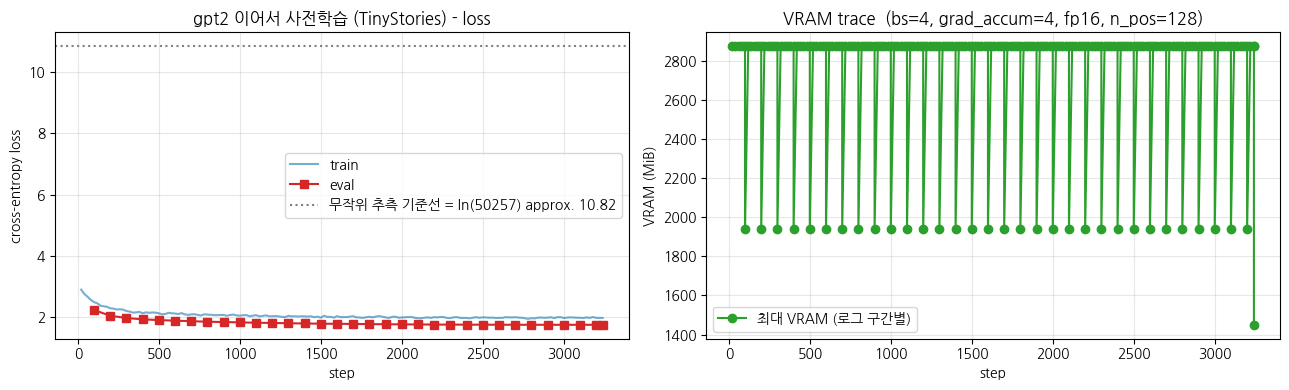
\includegraphics[width=0.88\linewidth]{assets/figures/ch25_loss_vram_trace.png}
\end{bookfigurelabel}

\textbf{그림 읽기} --- 그림~\ref{fig:ch25-loss-vram-trace}에서 다음 내용을 확인합니다: GPT-2 continual pretraining 손실과 VRAM 추적. 실행된 노트북에서 저장된 최신 plot 출력이므로, 코드에서 계산한 값이 어떤 평가 지점으로 이어지는지 바로 확인할 수 있습니다.



\textbf{관전 포인트} --- \ref{ch:24}장과 달리 \emph{첫 step loss 가 random baseline \texttt{ln(50257)\ ≈\ 10.82} 부근이 아니라 약 3.0-4.0 부근} 에서 시작합니다. \emph{gpt2 가 이미 일반 영어 분포를 학습해 둔 덕분에 TinyStories 평가에서도 시작 loss 가 낮음}. 학습 진행과 함께 약 2.0-2.5 로 더 떨어지는데, 이게 \emph{TinyStories 도메인 적응} 의 효과. 곡선이 \emph{random baseline 으로부터 빠르게 떨어지는 \ref{ch:24}장} vs \emph{이미 낮은 지점에서 시작해 천천히 더 떨어지는 \ref{ch:25}장} 의 모양 차이가 한눈에 보입니다.



\section{\texorpdfstring{학습 \emph{후} generation --- \emph{continual pretraining 의 효과}}{학습 후 generation --- continual pretraining 의 효과}}

같은 \inlinecode{PROMPTS\ /\ GEN\_KWARGS} 로 학습 후 모델에서 다시 생성. \emph{BEFORE (gpt2 그대로) \(\to\) AFTER (continual pretrained on TinyStories)} 비교가 \emph{학습 단계 2 가 본체에 새긴 도메인 적응} 을 직접 드러냅니다.



\textbf{해석 가이드 --- continual pretraining 의 도메인 적응 효과}

\begin{itemize}
\tightlist
\item
  \textbf{BEFORE (gpt2 그대로)}: 자연스러운 영어이지만 \emph{WebText 풍} --- 일반 산문 / 뉴스 / 대화 톤. \emph{Once upon a time} 같은 동화 도입에 대해서도 \emph{동화 스타일 이어쓰기보다 일반 산문 이어쓰기} 경향
\item
  \textbf{AFTER (gpt2 + TinyStories 1 epoch)}: 같은 prompt 가 \emph{동화 풍} 으로 이어짐 --- 짧고 단순한 문장, 동화 어휘 (little / mommy / friend / play / forest / happy ...), TinyStories 특유의 \emph{반복적이고 어린이 어휘 한정} 톤
\end{itemize}

\begin{quote}
본체는 \emph{같은 124M params 모델} 이고, \emph{한 줄 코드 차이 (lr) + 한 epoch 의 데이터} 만으로 \emph{generation 톤 자체가 도메인 적응}. 그게 \emph{continual pretraining 의 정량적 가치} --- \emph{task adaptation 의미의 fine-tune (head 교체 / 새 loss) 이 아닙니다}, \emph{같은 task 의 데이터만 바뀐 단계 1 의 연장}.
\end{quote}



\section{3-way generation 비교 --- \ref{ch:24}장 (scratch) vs \ref{ch:25}장 BEFORE vs \ref{ch:25}장 AFTER}

\ref{ch:24}장의 \emph{작은 from-scratch 모델} (3M, TinyStories 1500 step) 의 generation 결과를 \emph{옆에 두고} 비교합니다. \emph{\ref{ch:24}장 노트북 §7 의 “TRAINED model” generation 출력} 을 직접 인용 (사용자가 본인 결과로 갱신 가능).

\subsection{세 셋업의 차이}

\begin{booktable}{25장 세 셋업의 차이 표}{tab:ch25-09}
\begin{adjustbox}{max width=\textwidth}
\begin{tabular}{@{}llll@{}}
\toprule
셋업 & 본체 & 사전학습 & TinyStories 학습 \\
\midrule

\ref{ch:24}장 (scratch) & 3M params, random init & 없음 (from scratch) & 1500 step 사전학습 자체 \\
\textbf{\ref{ch:25}장 BEFORE} & 124M params (gpt2) & \textbf{WebText 약 40GB} & 없음 (gpt2 그대로) \\
\textbf{\ref{ch:25}장 AFTER} & 124M params (gpt2) & \textbf{WebText 약 40GB} & \textbf{1 epoch continual pretraining} \\
\bottomrule
\end{tabular}
\end{adjustbox}
\end{booktable}



\textbf{해석 가이드 --- 세 셋업의 격차}

\begin{itemize}
\tightlist
\item
  \textbf{\ref{ch:24}장 (3M scratch, TinyStories 1500 step)}: \emph{동화 풍 단순 영어} 가능 --- 작은 모델·작은 데이터로도 grammatical 한 생성. 다만 어휘는 동화 도메인에 한정
\item
  \textbf{\ref{ch:25}장 BEFORE (gpt2 그대로)}: \emph{다양한 도메인 영어} 가능. 자연스러운 산문이지만 \emph{TinyStories 풍은 아님}
\item
  \textbf{\ref{ch:25}장 AFTER (gpt2 + TinyStories continual pretrain)}: \emph{동화 풍 + 자연스러움 + 일반 도메인 어휘력} 결합. \emph{작은 from-scratch 의 도메인 특화 + 큰 사전학습 모델의 어휘 폭} 이 모두
\end{itemize}

\begin{quote}
\textbf{세 셋업의 비교가 던지는 질문} --- \ref{ch:25}장 AFTER 가 \ref{ch:24}장보다 \emph{훨씬 좋아 보인다면}, 이게 \emph{모델 크기 (3M \(\to\) 124M, 약 40배) 의 위력인가, 사전학습 (WebText 약 40GB) 의 위력인가?} --- 본 장의 셋업으로는 \emph{분리 불가능}. 두 요인이 \emph{함께 변함}. FAQ Q3 에서 더 자세히.
\end{quote}



\section{학습 곡선 비교 --- \ref{ch:24}장 vs \ref{ch:25}장의 학습 효율}

\emph{같은 데이터 (TinyStories 30K)} 에 대한 \emph{random init vs 사전학습 본체} 의 학습 효율 격차를 표로 정리.

\begin{booktable}{25장 학습 곡선 비교 - 24장 vs 25장의 학습 효율 표}{tab:ch25-10}
\begin{adjustbox}{max width=\textwidth}
\begin{tabular}{@{}lll@{}}
\toprule
항목 & \ref{ch:24}장 (3M scratch) & \textbf{\ref{ch:25}장 (124M continual pretrain)} \\
\midrule

시작 loss & 약 7.62 (\inlinecode{ln(2048)}, random baseline) & \textbf{약 3.0-4.0} (gpt2 pretrained, TinyStories 평가) \\
도달 loss (학습 끝, 누적 평균 \inlinecode{train\_loss}) & 약 3.8 & \textbf{약 2.07} \\
학습 step & 1,500 & \textbf{약 3,200} (1 epoch, 51,863 chunks / eff. batch 16) \\
학습 시간 (T4) & 약 1분 & \textbf{약 19분} \\
Vocab 차원 & 2,048 & \textbf{50,257} (loss 단위 다름 --- 직접 비교 어려움) \\
Generation 품질 & grammatical 한 동화 & \textbf{자연스러운 동화 + 일반 도메인 어휘} \\
\bottomrule
\end{tabular}
\end{adjustbox}
\end{booktable}

\begin{quote}
\textbf{요점}: \ref{ch:25}장은 \emph{시작부터 낮은 loss} 에서 출발해 더 낮은 지점까지 내려갑니다 --- 사전학습된 본체의 \emph{시작 이점}. step·시간은 \ref{ch:24}장보다 오히려 더 큽니다 (124M 본체 + chunk 수가 많아 1 epoch 이 길어짐). 다만 \emph{loss 의 절대값} 은 vocab 단위가 달라 직접 비교 어려움 (vocab 25배 차이). \emph{Generation 품질} 로는 §7 의 3-way 비교가 정성적 차이를 보여줍니다.
\end{quote}

\begin{quote}
\ref{ch:25}장의 결과만 보면 \emph{대규모 사전학습 + continual pretraining} 이 압도적으로 보이지만, \emph{3M params + WebText 사전학습} (가상의 비교군) 이라면 어떻게 될까요 --- \emph{모델 크기와 사전학습 데이터를 분리하는 비교} 는 본 장의 셋업으로는 어렵습니다. 그게 \emph{실험 설계의 한계} 이자 \emph{학습 단계 2 의 실용성} --- 실무는 보통 \emph{큰 사전학습 모델을 그대로 가져와 continual pretraining} 하는 게 비용 대비 최선이라.
\end{quote}



\section{변형: 더 많은 epoch / 다른 도메인 / catastrophic forgetting 시연}

본 장에서 다루지 못한 변형들 --- 직접 시도해 보고 싶다면 아래 코드를 출발점으로:

\subsection{\texorpdfstring{변형 1. epoch 수 늘리기 --- \emph{언제 catastrophic forgetting 이 시작되는가}}{변형 1. epoch 수 늘리기 --- 언제 catastrophic forgetting 이 시작되는가}}

\Needspace{5\baselineskip}
\begin{lstlisting}

\end{lstlisting}

\subsection{변형 2. 더 큰 본체 (gpt2-medium, 355M)}

\Needspace{5\baselineskip}
\begin{lstlisting}
# model = AutoModelForCausalLM.from_pretrained("gpt2-medium")
# 355M
\end{lstlisting}

\subsection{\texorpdfstring{변형 3. 다른 도메인 데이터 --- \emph{continual pretraining 의 일반성}}{변형 3. 다른 도메인 데이터 --- continual pretraining 의 일반성}}

\Needspace{5\baselineskip}
\begin{lstlisting}
# raw_train = load_dataset("bigcode/the-stack-smol", 
# data_dir="data/python", split="train[:5000]")
\end{lstlisting}

\subsection{변형 4. catastrophic forgetting 직접 확인}

\Needspace{5\baselineskip}
\begin{lstlisting}

\end{lstlisting}



\section{이 장에 등장한 라이브러리·함수}

\begin{booktable}{25장 새로 등장한 라이브러리}{tab:ch25-11}
\begin{adjustbox}{max width=\textwidth}
\begin{tabular}{@{}lll@{}}
\toprule
이름 & 한 줄 설명 & \ref{ch:24}장과 공유? \\
\midrule

\inlinecode{AutoModelForCausalLM.from\_pretrained("gpt2")} & OpenAI gpt2 (124M, WebText 사전학습) 본체 로드 & \textbf{새로 등장} (\ref{ch:24}장은 \inlinecode{GPT2LMHeadModel(config)} random init) \\
\inlinecode{AutoTokenizer.from\_pretrained("gpt2")} & gpt2 BPE 토크나이저 (vocab 50,257) 로드 & \textbf{새로 등장} (\ref{ch:24}장은 직접 학습 BPE) \\
\inlinecode{tokenizer.pad\_token\ =\ tokenizer.eos\_token} & gpt2 의 pad 컨벤션 (EOS 재활용) & \textbf{새로 등장} (\ref{ch:24}장은 PreTrainedTokenizerFast 인자로 직접 지정) \\
\inlinecode{transformers.Trainer} & HuggingFace 표준 학습 루프 & \textbf{공유} (\ref{ch:24}장과 동일 클래스, 동일 인자 구조) \\
\inlinecode{DataCollatorForLanguageModeling(mlm=False)} & CausalLM collator (\inlinecode{labels\ =\ input\_ids.clone()} 자동) & \textbf{공유} (\ref{ch:24}장과 정확히 같음) \\
\inlinecode{group\_texts} 패턴 (HF run\_clm.py 표준) & 가변 길이 텍스트 \(\to\) 고정 길이 블록 스트림 & \textbf{공유} \\
\inlinecode{model.generate(do\_sample=True,\ ...)} & sampling-based text generation & \textbf{공유} \\
\inlinecode{warmup\_ratio} (vs \inlinecode{warmup\_steps}) & epoch 비율 기반 warmup (continual pretraining 표준) & \textbf{약간 다름} (\ref{ch:24}장은 \inlinecode{warmup\_steps=100}) \\
\inlinecode{num\_train\_epochs} (vs \inlinecode{max\_steps}) & epoch 수 기반 학습 (continual pretraining 1 epoch 충분) & \textbf{약간 다름} (\ref{ch:24}장은 \inlinecode{max\_steps=1500}) \\
\inlinecode{gradient\_accumulation\_steps} & 작은 배치를 누적해 큰 effective batch (T4 + 124M 메모리 제약) & \textbf{새로 등장} (\ref{ch:24}장은 3M 이라 불필요) \\
\bottomrule
\end{tabular}
\end{adjustbox}
\end{booktable}



\section{체크포인트 질문}

\begin{enumerate}
\def\labelenumi{\arabic{enumi}.}
\tightlist
\item
  \ref{ch:24}장의 학습 첫 step loss 는 약 \texttt{ln(2048)\ ≈\ 7.62} 에서 시작했습니다. \ref{ch:25}장은 random baseline 이 \texttt{ln(50257)\ ≈\ 10.82} 인데 \emph{시작 loss 가 약 3.0-4.0} 입니다. 두 장의 \emph{시작 loss 차이} 가 의미하는 바는 무엇인가요? (랜덤 추측 / 사전학습된 본체 / vocab 차원의 관계)
\item
  본 장의 lr (\inlinecode{2e-5}) 가 \ref{ch:24}장의 lr (\inlinecode{3e-4}) 보다 \emph{약 15배 작은} 이유를 \emph{catastrophic forgetting} 키워드로 설명해 보세요. 만약 \ref{ch:25}장에서도 \inlinecode{3e-4} 를 썼다면 무슨 일이 일어날까요?
\item
  \emph{Continual pretraining} (단계 2, 본 장) 과 \emph{SFT} (단계 3, \ref{ch:28}장) 의 가장 큰 차이는 \emph{\inlinecode{labels\ =\ -100} 자리} 입니다. 본 장의 collator 가 만드는 \inlinecode{labels} 패턴과, \ref{ch:28}장에서 등장할 \texttt{labels{[}:prompt\_len{]}\ =\ -100} 한 줄의 차이를 직접 비교해 설명해 보세요.
\item
  \ref{ch:25}장 AFTER 의 generation 이 \ref{ch:24}장보다 좋아 보인다면, \emph{모델 크기 (3M \(\to\) 124M)} 의 효과인가 \emph{사전학습 데이터 (없음 \(\to\) WebText 40GB)} 의 효과인가? 본 장의 실험 셋업으로는 둘을 분리할 수 있나요? (분리하려면 어떤 추가 실험이 필요할까요?)
\end{enumerate}



\section{FAQ}

\begin{faqBox}{Q1. (이론) \emph{Continual pretraining} 이 정확히 무엇인가요? \emph{fine-tune} 과 어떻게 다른가요?}

\textbf{Continual pretraining} (계속 사전학습 / continual learning) 은 GPT 시대 학습 4단계 중 \emph{단계 2}:

\begin{booktable}{25장 FAQ 표}{tab:ch25-12}
\begin{adjustbox}{max width=\textwidth}
\begin{tabular}{@{}lll@{}}
\toprule
단계 & 정확 용어 & 의미 \\
\midrule

1 & \textbf{Pretraining} & random init 본체 + 일반 코퍼스 \\
2 & \textbf{Continual pretraining} \(\leftarrow\) \emph{본 장} & \emph{사전학습된 본체} + \emph{새 도메인 데이터}. \textbf{head 그대로, task 그대로, loss 그대로} \\
3 & \textbf{SFT} (Instruction tuning) & instruction-response 쌍, \texttt{labels{[}:prompt\_len{]}\ =\ -100} \\
4 & \textbf{Alignment} (DPO / RLHF / GRPO) & preference 또는 verifier reward \\
\bottomrule
\end{tabular}
\end{adjustbox}
\end{booktable}

\textbf{\inlinecode{fine-tune} 이라는 단어는 \emph{세 의미가 섞여 쓰입니다}}:

\begin{itemize}
\tightlist
\item
  \textbf{BERT 단계 fine-tune}: \emph{task adaptation} --- 본체 + 새 head (\inlinecode{Linear(H,\ K)}) + 새 task loss. \ref{ch:09}--\ref{ch:23}장의 분류 장들.
\item
  \textbf{GPT 시대 continual pretraining}: \emph{데이터 적응} --- 본체 + 같은 head + 같은 loss + 새 데이터. \textbf{본 장.}
\item
  \textbf{GPT 시대 SFT}: \emph{행동 정렬} --- 본체 + 같은 head + 같은 loss + instruction-response 데이터 + \inlinecode{-100} 마스킹. \ref{ch:28}장.
\end{itemize}

정확히 부르자면 본 장은 \emph{fine-tune 이 아니라 continual pretraining}. \emph{task 가 안 바뀌고 데이터만 바뀐} 게 핵심.

\end{faqBox}

\begin{faqBox}{Q2. (실무) 왜 lr 가 \ref{ch:24}장의 \inlinecode{3e-4} 보다 작은 \inlinecode{2e-5} 인가요?}

\textbf{catastrophic forgetting 방지} 가 핵심 이유. \emph{사전학습된 본체} 는 weight 들이 \emph{이미 의미 있는 표상} 을 학습한 상태. 큰 lr 로 학습하면:

\begin{enumerate}
\def\labelenumi{\arabic{enumi}.}
\tightlist
\item
  \emph{사전학습된 표상이 새 데이터에 맞춰 크게 흔들림}
\item
  \emph{원래 알던 일반 도메인 지식 (WebText 풍 영어 전반)} 이 \emph{TinyStories 동화 풍} 으로 \emph{덮어쓰기}
\item
  결과: \emph{TinyStories 도메인은 잘 하지만 일반 영어 능력 손실} --- 이게 catastrophic forgetting
\end{enumerate}

작은 lr (\inlinecode{2e-5}) 는 \emph{사전학습된 표상 보존} 을 우선합니다. \emph{기존 weight 에서 살짝만 떨어진 지점으로 이동} --- 도메인 적응은 하되 일반 능력은 유지.

\Needspace{5\baselineskip}
\begin{lstlisting}
TrainingArguments(learning_rate=3e-4, ...)

TrainingArguments(learning_rate=2e-5, ...)
\end{lstlisting}

HF 의 continual pretraining / fine-tuning 표준 lr 범위: \inlinecode{1e-5} - \inlinecode{5e-5}. SFT (\ref{ch:28}장) 도 비슷한 범위.

\end{faqBox}



\begin{faqBox}{Q5. (이론·실무) \emph{catastrophic forgetting} 이 무엇인가요? \ref{ch:25}장에서 실제로 일어나나요?}

\textbf{Catastrophic forgetting} (재앙적 망각): 새 데이터로 학습할 때 \emph{이전에 학습한 표상이 덮어쓰기} 되어 \emph{원래 알던 능력이 손실} 되는 현상.

\ref{ch:25}장에서는 \emph{짧은 (1 epoch) continual pretraining + 작은 lr (\inlinecode{2e-5})} 라 \emph{catastrophic forgetting 이 강하지 않음}. 다만 \emph{변형 1 (epoch 늘리기)} 또는 \emph{큰 lr (\inlinecode{1e-3} 등)} 을 시도하면 다음 신호가 보입니다:

\begin{itemize}
\tightlist
\item
  비-동화 prompt (예: \inlinecode{"Albert\ Einstein\ was\ a"}) 에 대해 \emph{gpt2 가 원래 답했을 만한 일반 영어} 가 \emph{동화풍 톤} 으로 끌려감
\item
  \emph{generation 다양성 하락} --- 모든 prompt 에 \emph{little / mommy / friend} 류 동화 단어가 자주 등장
\item
  \emph{evaluation} --- 만약 GLUE 같은 일반 영어 벤치마크에 \emph{학습 전 / 후} 를 측정하면 \emph{학습 후가 더 낮은 점수}
\end{itemize}

방지법:

\begin{enumerate}
\def\labelenumi{\arabic{enumi}.}
\tightlist
\item
  \textbf{짧은 학습 + 작은 lr} (본 장 패턴)
\item
  \textbf{regularization} --- replay (이전 데이터 일부 섞어 학습) / EWC (Elastic Weight Consolidation) 등
\item
  \textbf{adapter / LoRA} --- 본체 weight 는 freeze 하고 작은 adapter 만 학습 \(\to\) 본체 표상 보존
\end{enumerate}

본 장은 \emph{방법 1} 만 적용. \emph{방법 3 (LoRA)} 는 본 커리큘럼 범위 밖이지만 \emph{실무에서는 표준 옵션}.

\end{faqBox}





\compactFAQMore{4}

\begin{previewBox}{미리보기: 다음 장}

\textbf{\ref{ch:26}장. 한국어 작은 GPT scratch --- \emph{\ref{ch:24}장의 한국어판}}

\begin{itemize}
\tightlist
\item
  \inlinecode{roneneldan/TinyStories} 의 한국어 짝 (TinyStories-Korean 또는 유사 한국어 동화 데이터셋) 으로 \emph{한국어 GPT scratch} 학습
\item
  \emph{한국어 BPE 직접 학습} --- gpt2 BPE 가 한국어를 못 다루는 이유 (Q4 참고) 를 출발점으로, 한국어 코퍼스 위에 새 BPE 학습
\item
  \emph{작은 GPT2LMHeadModel(config)} random init --- \ref{ch:24}장과 \emph{같은 패턴, 데이터 + 토크나이저만 한국어}
\item
  비교: \ref{ch:22}장 (한국어 BERT scratch) 와 같은 한국어 사전학습 단계 1 이지만 \emph{encoder MLM \(\to\) decoder CausalLM}
\end{itemize}

\textbf{Phase 4 GPT 시대 4단계 흐름 정리}:

\begin{booktable}{25장 FAQ 표}{tab:ch25-15}
\begin{adjustbox}{max width=\textwidth}
\begin{tabular}{@{}lllll@{}}
\toprule
장 & 단계 & 본체 & 데이터 & 핵심 \\
\midrule

\ref{ch:24}장 & 1 (영어) & 작은 GPT scratch & TinyStories & 단계 1 출발 \\
\textbf{\ref{ch:25}장 \(\leftarrow\) 여기} & \textbf{2} & \textbf{\inlinecode{gpt2} 124M} & \textbf{TinyStories (동일)} & \textbf{단계 2: continual pretraining} \\
\ref{ch:26}장 & 1 (한국어) & 작은 GPT scratch & TinyStories-Korean & 한국어 단계 1 \\
\ref{ch:27}장 & 2 (한국어) & KoGPT2 125M & TinyStories-Korean & \textbf{한국어 단계 2: continual pretraining} (본 장의 한국어 짝) \\
\ref{ch:28}장 & 3 & KoGPT2 + SFT & KoAlpaca 등 instruction 데이터 & \textbf{단계 3: SFT} \\
\ref{ch:30}장 & 4 & SFT 모델 + DPO & preference 쌍 데이터 & \textbf{단계 4: DPO} \\
\ref{ch:31}장 & 4 & SFT 모델 + GRPO & verifier reward & \textbf{단계 4: GRPO} \\
\bottomrule
\end{tabular}
\end{adjustbox}
\end{booktable}

\begin{quote}
\emph{왜 영어 사전학습 모델 (gpt2) 을 한국어에 그대로 적용하기 어려운가} 의 답이 \ref{ch:26}장의 동기입니다 --- \emph{토크나이저가 한국어를 못 다루면 본체 weight 가 유효한 신호가 아니라} 사실상 random init 과 같은 상태. 한국어는 \emph{처음부터} 가 정공법.
\end{quote}

\begin{quote}
\textbf{변하는 축} (\ref{ch:25}장 \(\to\) \ref{ch:26}장): \emph{언어 + 학습 단계} 두 축. \emph{직접 짝} 은 \ref{ch:24}장 \(\leftrightarrow\) \ref{ch:26}장 (같은 단계 1, 언어만 다름) / \textbf{\ref{ch:25}장 \(\leftrightarrow\) \ref{ch:27}장} (같은 단계 2 continual pretraining, KoGPT2 + 한국어 TinyStories) 입니다. 영어·한국어가 \emph{scratch + continual pretraining} 으로 완전 대칭.
\end{quote}
\end{previewBox}



\section{보조 시각화}

\begin{bookfigurelabel}[H]{TinyStories CLM의 scratch 학습과 continual pretraining 손실 비교}{fig:ch25-ch24-loss-compare}
\centering
\includegraphics[width=0.72\linewidth]{assets/figures/ch25_ch24_loss_compare.png}
\end{bookfigurelabel}

\textbf{그림 읽기} --- 그림~\ref{fig:ch25-ch24-loss-compare}에서 다음 내용을 확인합니다: TinyStories CLM의 scratch 학습과 continual pretraining 손실 비교. 실행된 노트북에서 저장된 최신 plot 출력이므로, 코드에서 계산한 값이 어떤 평가 지점으로 이어지는지 바로 확인할 수 있습니다.